\documentclass[11pt,a4paper]{article}
\usepackage[utf8]{inputenc}
\usepackage[english]{babel}
\usepackage{amsmath}
\usepackage{amsfonts}
\usepackage{amssymb}
\usepackage{mathrsfs}
\usepackage{gensymb}
\usepackage{fancyhdr}
\usepackage[left=1.5cm,right=1.5cm,top=2.5cm,bottom=2cm]{geometry}
\usepackage{adjustbox}
\usepackage{booktabs}  
\usepackage{threeparttable} 
\usepackage{makecell}
\usepackage{parskip}
\usepackage{graphicx}
\usepackage{listings}


\begin{document}
\title{MCMC Sampling Methods}
\pagestyle{fancy}

{
\fancyhf{}
\rhead{11 June 2018}
\lhead{Yunzhe Li, Yizi Zhang, Ruriko Imai} 
\cfoot{\thepage}
}

\vspace*{\fill}
\begin{center}
\subsection*{ 
\huge Comparing Metropolis and Gibbs Sampling Method
}
\end{center}

\begin{center}
Yunzhe Li: madli@ucdavis.edu \\
Ruriko Imai: raimai@ucdavis.edu \\
Yizi Zhang: yizzhang@ucdavis.edu
\end{center}
\bigskip
\bigskip
\bigskip
\bigskip
\bigskip
\bigskip
\bigskip
\bigskip
\bigskip
\bigskip
\bigskip
\bigskip


\begin{center}
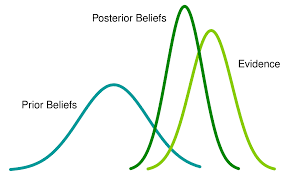
\includegraphics[scale=1.5]{images/cover.png}
\end{center}
\vspace*{\fill}
\newpage

\section*{Introduction}
The purpose of this project is to explore sampling methods derived from algorithms in the Monte Carlo Markov Chain (MCMC) family called the Metropolis sampling and Gibbs sampling methods. These MCMC algorithms are used in a bayesian setting where direct sampling from the posterior distribution is difficult. By sampling from the posterior we will be able to estimate mean and other parameters to further analyze the data. In order to check for performance, speed and accuracy of those sampling methods, we shall use a known posterior distribution so the distribution obtained from Metropolis and Gibbs sampling methods can be compared. Therefore, the  setting of the sampling distribution is Multinomial - Dirichlet conjugate with K = 3 categories with two-dimensional parameters to update. 

\section*{Difference between Gibbs and Metropolis Algorithm}
Metropolis-Hastings sampler is the umbrella algorithm for both Gibbs and Metropolis sampling methods. These sampling methods are used when direct sampling is deemed difficult to perform on a given posterior distribution. Gibbs sampling is a special case of Metropolis hastings algorithm with a probability acceptance rate of 1. Metropolis sampling is also a special case of Metropolis hastings, requiring a symmetric proposal distribution. Although the algorithms are slightly different, the purpose is to sample from the posterior distribution. 
\newline
Some issues to consider are: 
 
\begin{itemize}
 \item determine a good burn-in amount to decrease dependence on starting values  
 \item determine a good thinning amount to decrease autocorrelation
 \item determine a good proposal distribution for Metropolis sampler
 \item partial correlation between parameters
 \item convergence diagnostics
\end{itemize}
 
We will explore these issues throughout this simulation process.	


\section*{Set-Up}
\begin{itemize}
	\item Data: 
	\begin{itemize}
		\item True parameters: $\theta_{1} = 0.1$, $\theta_{2} = 0.7$, $\theta_{3} = 0.2$
		\item Hyperparameters: $\alpha_{1} = 2$, $\alpha_{2} = 2$, $\alpha_{3} = 2$ 
	\end{itemize}
	\item Prior: $X_{i} | \theta \overset{H_0}{\sim} Multinom(n, \theta_{1}, \theta_{2}, \theta_{3}); i = 1, \dots, n$
\end{itemize}

\end{document}